\section{Area e volume}
L'area è definita nel sistema internazionale come la misura della superficie rispetto all'unità di riferimento (il metro quadro, simbolo $\si{\square\meter}$, figura  \ref{fig:quad}), ossia un quadrato di lato 1 m. Il volume invece è definito come la misura dello spazio occupato da un corpo rispetto all'unità di misura base, un cubo di lato un metro, il metro cubo (simbolo $\si{\cubic\meter}$, figura \ref{fig:cub})\\

\begin{minipage}{\linewidth}
	\centering
	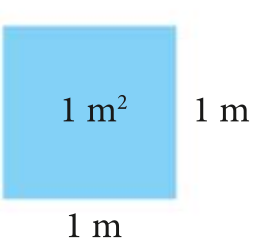
\includegraphics[scale=0.3]{quad}
	\captionof{figure}{Il metro quadro}
	\label{fig:quad}
\end{minipage}
\begin{minipage}{\linewidth}
	\centering
	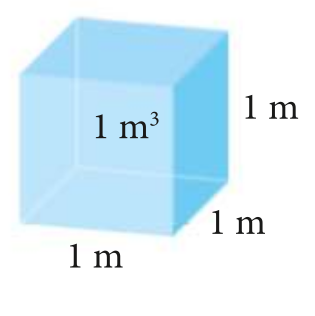
\includegraphics[scale=0.3]{cub}
	\captionof{figure}{Il metro cubo}
	\label{fig:cub}
\end{minipage}


Poichè queste due grandezze non fanno parte delle 7 grandezze fondamentali, si chiamano \textit{derivate}. I multipli di \(\si{\square\meter}\) sono quadrati con lati di lunghezza \(\SI{1}{\deca\meter}\) (\(\si{\square\deca\meter}\), decametro quadro), \(\SI{1}{\hecto\meter}\) (\(\si{\square\hecto\meter}\), ettometro quadro), \(\SI{1}{\kilo\meter}\) (\(\si{\square\kilo\meter}\), chilometro quadro), mentre i sottomultipli sono quadrati di lato \(\SI{1}{\deci\meter}\) (\(\si{\square\deci\meter}\), decimetro quadro), \(\SI{1}{\centi\meter}\) (\(\si{\square\centi\meter}\), centimetro quadro), \(\SI{1}{\milli\meter}\)\ (\(\si{\square\milli\meter}\), millimetro quadro). Analogamente per il volume: \(\si{\cubic\deca\meter}\) (decametro cubo), \(\si{\cubic\deci\meter}\) (decimetro cubo), ecc.


Le  equivalenze con questa grandezze si riducono a quelle lineari (basta contare i quadrati o i cubi contenuti) per andare dal multiplo a sottomultiplo). Per andare da sottomultipli a  multipli, basta dividere per un'opportuna potenza di 10. Vediamo un esempio: \,$\SI{1,5}{\cubic\meter} = \cdots \si{\cubic\centi\meter}$. Un cubo di lato $\SI{1}{\cubic\meter}$ contiene su ogni lato, 100 cm (oppure 10 dm, vedi  figura \ref{fig:da-m3-a-cm3}), dunque $\SI{1}{\cubic\meter} = 100\times100\times100 = \SI{e+6}{\cubic\centi\meter}$, per cui:
\[
\SI{1,5}{\cubic\meter} = \SI{1,5e+6}{\cubic\centi\meter}
\]

\begin{minipage}{\linewidth}
	\centering
	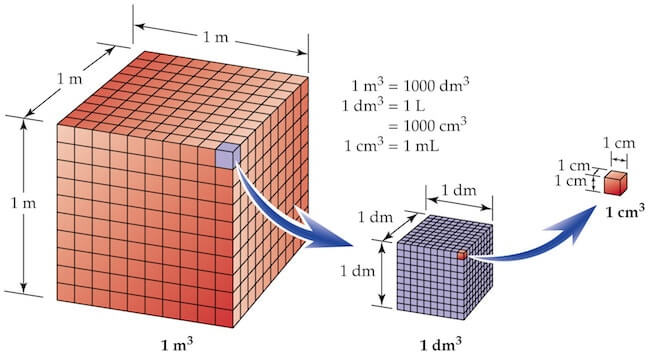
\includegraphics[scale=0.5]{da-m3-a-cm3}
	\captionof{figure}{Suddivisione di $\SI{1}{\cubic\meter}$ in cubi di lato 1 dm e 1 cm}
	\label{fig:da-m3-a-cm3}
\end{minipage}






Altro esempio: $\SI{1200}{\cubic\deci\meter} = \cdots \si{\cubic\meter}$.

Poichè 1 metro cubo contiene  $10\times10\times10 = \SI{e3}{\cubic\deci\meter}$,   e poiché   nella nostra equivalenza andiamo da sottomultiplo a multiplo, dobbiamo dividere per $10^3$:
\[
\SI{1200}{\cubic\deci\meter} = \frac{1200}{10^3}\,\si{\cubic\meter} = \SI{1,2}{\cubic\meter}.
\]

Nella pratica dei laboratori, si incontra il litro, simbolo L, definito come un decimetro cubo. Proviamo a risolvere l'equivalenza: $\SI{1}{\cubic\centi\meter} =\cdots \si{\milli\liter}$. In questi casi, conviene trasformare in litri e poi da litri a millilitri:
\[
\SI{1}{\cubic\centi\meter} = \SI{e-3}{\cubic\deci\meter}= \SI{e-3}{\liter}=10^{-3}\times\SI{e+3}{\milli\liter} =\SI{1}{\milli\liter}.
\]
Abbiamo usato la regola seguente: se tra due multipli lineari c'è una potenza di 10 $``N''$, tra i cubi c'è una potenza $3 N$. Poiché tra centimetri e decimetri c'è solo una potenza $10^1$, allora tra i cubi c'è $10^3$. Si guardi a tal proposito la figura \ref{fig:equiv2}
\vspace{0.5cm}
\begin{minipage}{\linewidth}
	\centering
	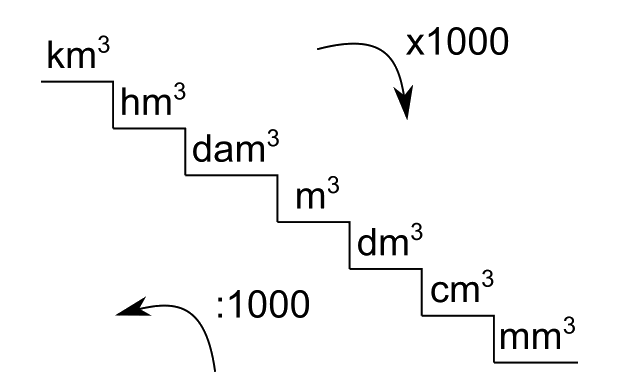
\includegraphics[scale=0.3]{equiv2}
	\captionof{figure}{Equivalenze tra volumi}
	\label{fig:equiv2}
\end{minipage}


Questa equivalenza è particolarmente importante per cui la mettiamo in edidenza:
\[
\colorboxed{ocre}{
\SI{1}{\cubic\centi\meter} = \SI{1}{\milli\liter}
}
\]
Risolviamo in fine una equivalenza con un'area: $\SI{2,34e+4}{\square\deci\meter} = \cdots \si{\square\deca\meter}$. In questo caso vale la regola del ''2'' ossia le potenze vanno moltiplicate per due:
\[
\SI{2,34e+4}{\square\deci\meter} = 2,34\times10^{4}\times 10^{-4}\,\si{\square\deca\meter} 
\]

